
%(BEGIN_QUESTION)
% Copyright 2012, Tony R. Kuphaldt, released under the Creative Commons Attribution License (v 1.0)
% This means you may do almost anything with this work of mine, so long as you give me proper credit

{\bf Isomerization feed flow control loop}

$$\includegraphics[width=15.5cm]{i0009rx01.eps}$$

\underbar{file i0009r}
%(END_QUESTION)





%(BEGIN_ANSWER)


%(END_ANSWER)





%(BEGIN_NOTES)


\filbreak \vskip 20pt \vbox{\hrule \hbox{\strut \vrule{} {\bf Virtual Troubleshooting} \vrule} \hrule}

\noindent
{\bf Predicting the effect of a given fault:} present each of the following faults to the students, one at a time, having them comment on all the effects each fault would produce.

\begin{itemize}
\item{} Pair 4 of cable ISOM-18 fails open
\item{} Resistor in FTA-HLAI fails open
\item{} Cable pair FT-733 at transmitter fails shorted
\end{itemize}


\vskip 10pt


\noindent
{\bf Identifying possible/impossible faults:} present symptoms to the students and then have them determine whether or not a series of suggested faults could account for all the symptoms, explaining {\it why} or {\it why not} for each proposed fault:

\begin{itemize}
\item{} Symptom: {\it FC-733 reads -25\% flow for process variable}
\item{} Incorrect LRV/URV range points in FT-733 -- {\bf No}
\item{} +24 VDC supply failed in FTA-HLAI -- {\bf Yes}
\item{} FI-733 indicator failed open -- {\bf No -- discuss role of diode!}
\item{} FT-733 diode (note 1) failed open -- {\bf No}
\item{} FT-733 resistor (note 1) failed open -- {\bf Yes}
\end{itemize}


\vskip 10pt


\noindent
{\bf Determining the utility of given diagnostic tests:} present symptoms to the students and then propose the following diagnostic tests one by one.  Students rate the value of each test, determining whether or not it would give useful information (i.e. tell us something we don't already know).  Students determine what different results for each test would indicate about the fault, if anything:

\begin{itemize}
\item{} Symptom: {\it FV-733 remains closed at all times regardless of FC-733's output value ; voltage between terminals 15 \& 16 = 0 volts}
\item{} Measure voltage between terminals 19 \& 20 -- {\bf Yes}
\item{} Measure voltage between FV-733 terminals -- {\bf No}
\item{} Measure voltage between terminals 25 \& 26 -- {\bf No}
\item{} Measure voltage between terminals 13 \& 14 -- {\bf No}
\item{} Measure current at terminal 19 -- {\bf Yes}
\item{} Measure current at terminal 26 -- {\bf Yes}
\end{itemize}


\vskip 10pt


\noindent
{\bf Diagnosing a fault based on given symptoms:} imagine a loose wire connection develops on the left-hand side of terminal 42 in this system (don't reveal the fault to students!).  Present the operator's observation(s) to the students, have them consider possible faults and diagnostic strategies, and then tell them the results of tests they propose based on the following symptoms, until they have properly identified the nature and location of the fault:

\begin{itemize}
\item{} Operator observation: {\it Flow registers -25\%}
\item{} $V_{13-14}$ (or closer to xmtr) = 0 volts
\item{} $V_{41-42}$ (or closer to FTA-HLAI) = 24 volts
\item{} $I$ = 0 mA (anywhere in series with the loop)
\end{itemize}

%INDEX% Documentation, loop diagram: realistic industrial example (shared by i03404 and i03891)

%(END_NOTES)

